\documentclass{jpreprint}
\usepackage{setspace}


\def\vector#1{\mbox{\boldmath{$#1$}}}

\jtitle{
コード進行および歌詞情報を用いた\\
楽曲分類システムの構築
}
\title{
Construction of Musical Compositions Classification Systems \\
Based on Chord Progressions and Lyrics
}
\jauthor{齋藤 佑樹}
\author{Yuki Saito}
\jcourse{電子情報システム工学専攻}
\course{Electronic and Information Systems Engineering}
\jlab{天元} % 研究室名(指導教員名)
% 以下の \abstract をコメントアウトすると1年生用フォーマットになります
\abstract{
  %\begin{spacing}{0.8}
  In this study,
  we aimed to construct musical compositions classification systems
  with chord progressions and lyrics. 
  We utilized Hidden Markov Model for modelizing chord progressions of musics.
  In order to estimate affective scores of tunes,
  we also applied morphological analysis to lyrics of them.
  We conducted the classification experiment 
  by using data on the Web for the purpose of evaluating our systems.
  %\end{spacing}
}
\keyword{machine learning}
\keyword{data mining}
\keyword{natural language processing}

\begin{document}
\maketitle

\begin{multicols}{2}
  
\section{はじめに}
コンピュータネットワークをはじめとした情報工学の分野における技術の発展により, 
大量の楽曲データを取り扱うことが可能となった.
本研究では, 楽曲のコード進行と歌詞情報の利用により,
楽曲の印象などをより正確に反映させることができる楽曲分類システムを構築する.
また,
インターネットを介して入手したデータに基づいた楽曲分類実験により,
本研究で構築したシステムの有効性を検証する.

\section{コード進行による楽曲のモデル化} 
\subsection{近親調に基づくコード進行の数値化}
本研究では, 
楽曲を構成するコード進行を音楽理論において定義されている
近親調\cite{NGSW07}に基づいて
数値化した.
近親調に基づいて類似している調の主音は
図\ref{fig:cof}に示す五度圏上で近接した配置になるという特徴があるため, 
本研究ではハ長調 (C major) およびイ短調 (A minor) を基準とした
五度圏上での主音の配置に基づいてコード進行の数値化を行なった.

\begin{figurehere}
  \centering
  \scalebox{0.2}{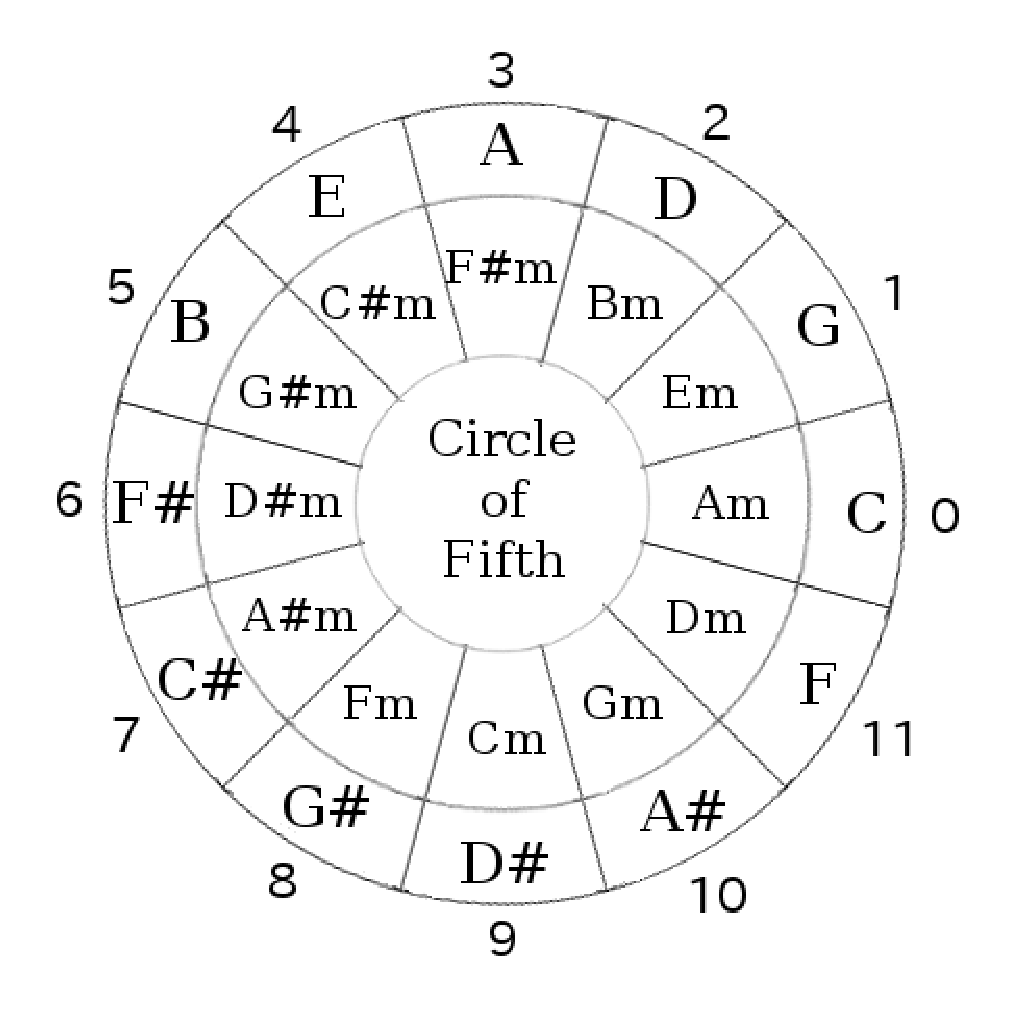
\includegraphics{cof.eps}}
  \vspace{-0.5cm}
  \caption{五度圏}
  \label{fig:cof}
\end{figurehere}

\subsection{HMM による楽曲のモデル化}
前節のとおりに数値化されたコード進行のデータを入力し,
Hidden Markov Model (HMM) の学習を行なった.
HMM は時系列で変化するデータをモデル化する際に用いられる手法であり,
入力データの変化を上手く表現するパラメータを学習により求める.
コード進行を構成するコードの役割は
トニック, ドミナント, サブドミナントという3つに大きく分けられるため,
本研究では HMM のトポロジーとして図~\ref{fig:hmm}に示す
状態数3の Ergodic HMM を採用した.

\vspace{0.25cm}
\begin{figurehere}
  \centering
  \scalebox{0.3}{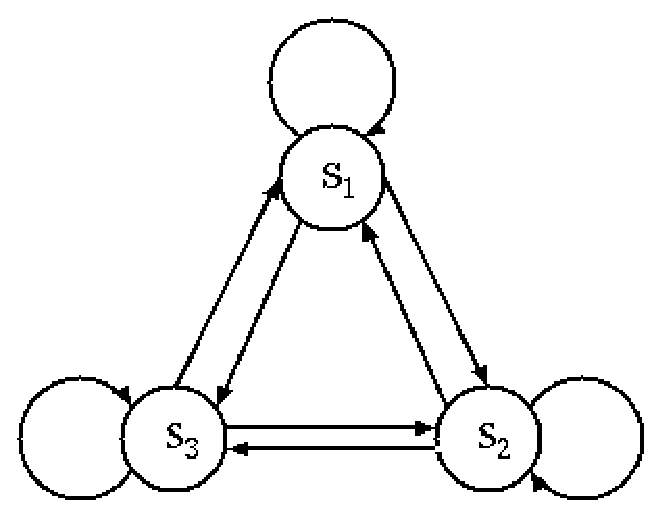
\includegraphics{hmm.eps}}
  \vspace{-0.5cm}
  \caption{Ergodic HMM のトポロジー}
  \label{fig:hmm}
\end{figurehere}

\section{歌詞情報を用いた楽曲の感情推定}
\subsection{感情スコアの定義}
本研究では感情のモデルとして
Robert Plutchikにより提唱されている「感情の輪」\cite{RP01} を用いた.
感情の輪は図\ref{fig:woe}に示すように,
感情を8つの基本感情 
(ecstasy, admiration, terror, amazement, grief, loathing, rage, vigilance)
の強弱と組合せで表現するものである.
本研究では感情の輪に存在する単語 (感情カテゴリ) に対し,
その位置に応じた感情スコアを8次元の数値ベクトルとして割り当てた.

\begin{figurehere}
  \centering
  \scalebox{0.3}{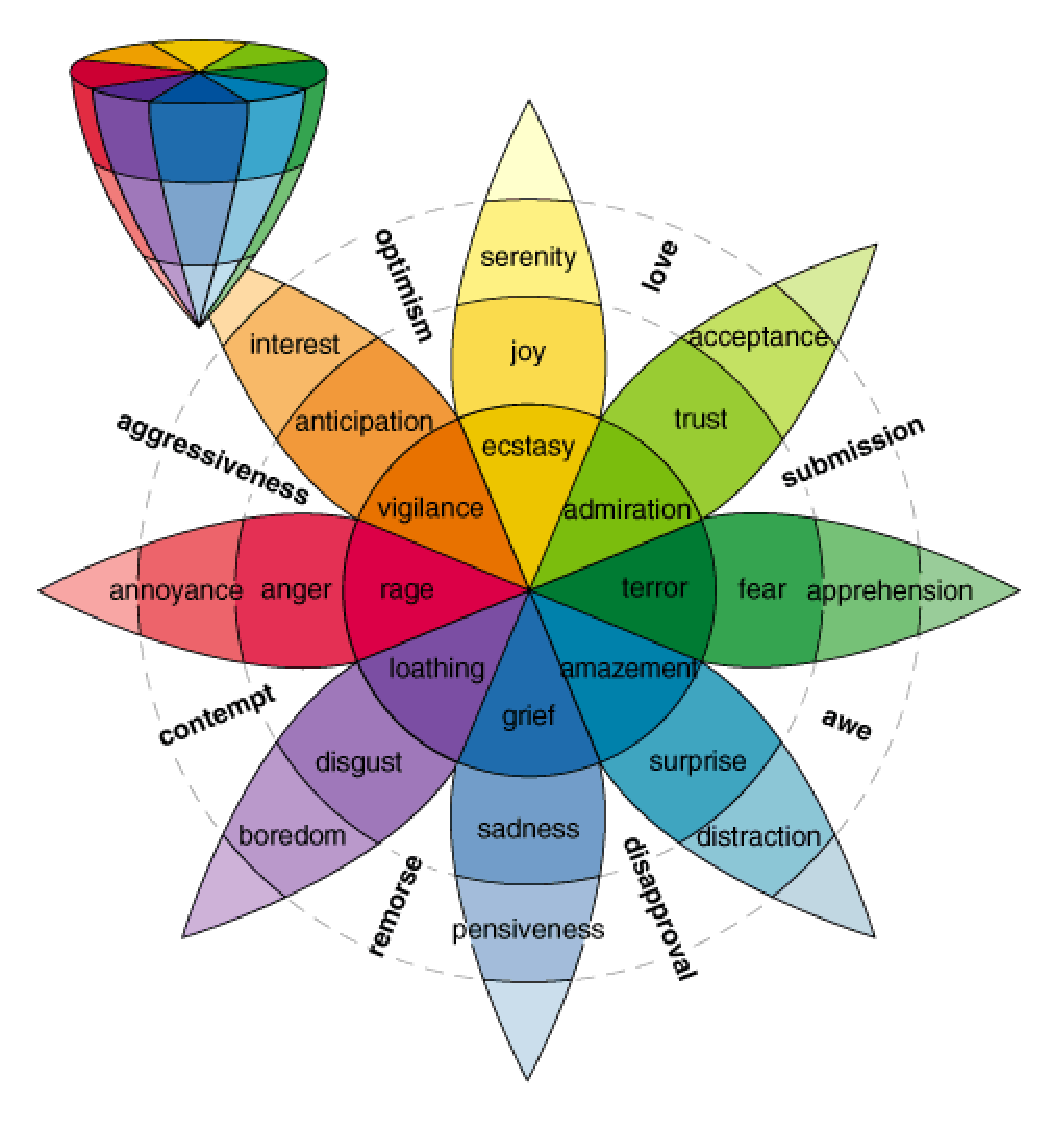
\includegraphics{woe.eps}}
  \vspace{-0.5cm}
  \caption{Plutchik の感情の輪}
  \label{fig:woe}
\end{figurehere}

\subsection{感情語辞書の作成}
楽曲の歌詞からの感情分析を行うために,
感情に関する語句 (感情語) を格納した感情語辞書を作成した.
感情語辞書は 
WordNet \cite{WN} から得られた単語をもとにして作成されており,
感情カテゴリと類似した意味を持つ単語
(下位語, 類義語, 派生系など) とその和訳を
含んでいる.
表\ref{tab:a_words}に感情語辞書に格納されている感情語の一例を示す.

\begin{tablehere}
  \caption{感情語の一例}
  \label{tab:a_words}
  \begin{tabular}{ccc}
    \hline
    \hline
    感情語 & 英訳 & 感情カテゴリ \\
    \hline
    好き & like & love \\
    臆病 & timidity & fear \\
    涙 & weepiness & sadness \\
    \hline
    \hline
  \end{tabular}
\end{tablehere}


\subsection{歌詞からの感情分析}
楽曲の歌詞に対して自然言語処理の手法を適用し,
その楽曲に対する感情分析を行なった.
以下に処理手順の概略を示す.
\begin{enumerate}
\renewcommand{\labelenumi}{(\arabic{enumi})}
\item 分類対象となる全ての楽曲の歌詞に対して形態素解析を行い, 感情語を抽出する.
\item 各感情語に対応する感情カテゴリを参照し, それに基づいて感情スコアを算出する.
\item 各感情スコアをtf-idfにより重み付けした値を楽曲に対する感情として推定する.
\end{enumerate}

\section{$k$-means 法による楽曲分類}
楽曲の分類を行うための手法として,
代表的な教師なし分類手法の1つである $k$-means 法を利用した.
本研究では, 
学習を終えた後の HMM のパラメータおよび
歌詞からの感情分析によって得られた感情スコアを特徴ベクトルとして
$k$-means 法による楽曲分類を行なった.

\section{分類実験とその結果}
本研究で構築した楽曲分類システムを評価するために楽曲の分類実験を行なった.
分類対象となるデータは 
J-Total Music\cite{JTM} 
から html ファイルとして入手したものを利用し,
分類のために必要な楽曲のコード進行および歌詞の情報と,
分類結果の正当性を判断するために利用する曲名, アーティスト名, 
楽曲のキーの情報を抽出した. 

\subsection{楽曲分類の結果}
クラスタ数を五度圏上に存在するすべての主音の個数である24として楽曲の分類実験を
行なった.
結果として,
各クラスタがそれぞれ五度圏上で近接した位置に存在する主音をキーとする楽曲の集まり
として構成されていることが確認された.

\subsection{感情分析の結果}
実際に楽曲の歌詞からの感情分析を行なった結果の一例を図\ref{fig:a_score}に示す.
この楽曲の歌詞は「愛情, 恋, 愛」などの 
"love" カテゴリに属する感情語を多く含んでおり, 
分析結果もそれに応じて ecstasy, admiration の
感情スコアが高まっていることが確認された.


\begin{figurehere}
  \centering
  \scalebox{0.4}{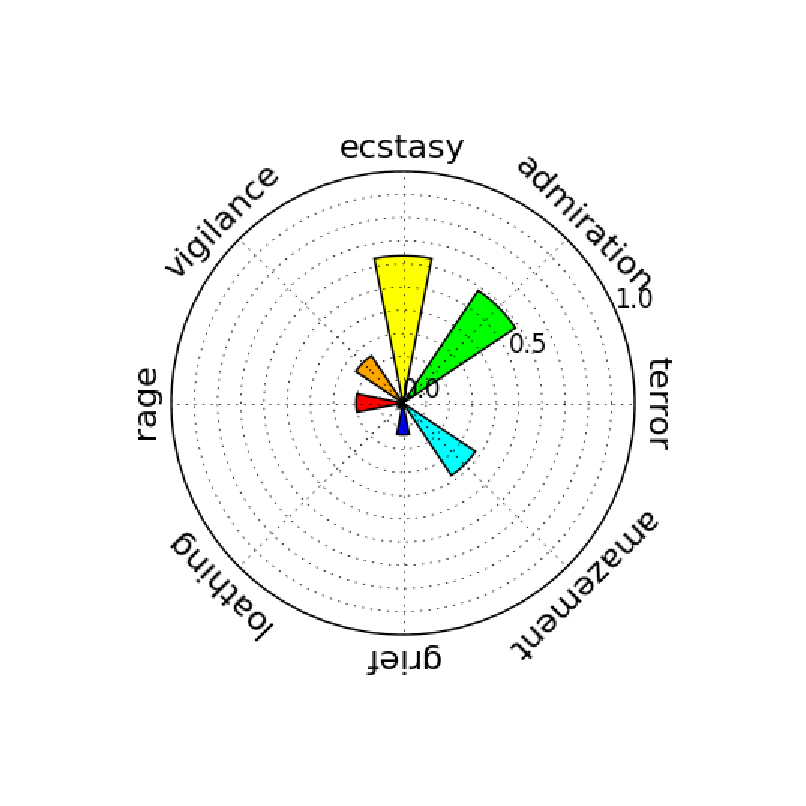
\includegraphics{a_score2.eps}}
  \vspace{-1.0cm}
  \caption{感情分析結果の一例}
  \label{fig:a_score}
\end{figurehere}

\section{おわりに}
本研究では, 
コード進行と歌詞情報の両方を利用して楽曲の分類を行うシステムを構築した.
今後はさらに歌詞からの感情分析結果を利用した楽曲検索を行う機能などを追加し,
より実用的な楽曲の分類および分析を行うシステムの実現を目指す.
%
% 以下に文献を書きます。
%

{\small
\begin{thebibliography}{99}
  \bibitem{NGSW07}
    長澤 槙子ほか, 
    “近親調を用いた楽曲クラスタリングシステムの構築に向けて”,
    電子情報通信学会第18回データ工学ワークショップ論文集, 2007.
  %\bibitem{FNSW09}
   % 舟澤 慎太郎ほか,
    %“歌詞の印象に基づく楽曲検索のための楽曲自動分類に関する検討”,
   % 情報処理学会第71回全国大会講演論文集, 2009.
  \bibitem{RP01}
    R. Plutchik,
    “\textit{The Nature of Emotions}”,
    American Scientist, Volume 89, Number 4, pp.344-350, 2001.
  \bibitem{WN}
    WordNet, “https://wordnet.princeton.edu/”
  \bibitem{JTM}
    J-Total Music, “http://music.j-total.net/”
\end{thebibliography}
}

\end{multicols}
\end{document}
